\begin{entry}{Q018}{Free-fermion brickwork circuit: from Jordan--Wigner to $\langle Z_x\rangle$}
 
\entrymeta{
  topic   = {Quantum circuits; Jordan--Wigner transformation; Bogoliubov rotation;
    Gaussian states and Wick's theorem; non-equilibrium many-body dynamics.},
  est     = {$\sim$90 minutes --- a multi-session entry. Natural split: (a) warm-up;
    (b)--(c) the fermionic and momentum representations; (d) the Floquet
    diagonalisation; (e) the observable.},
  origin  = {Adapted. Tutorial~1 of the course, restated so that it stands alone:
    the basis $\ket{\pm}$, the circuit geometry and the site labelling are made
    explicit, and the sign and labelling conventions (Jordan--Wigner string,
    momentum set, $A_k$ versus $B_k$) are fixed so that every displayed identity
    holds as written.},
  source  = {B. Bertini, \emph{Non-equilibrium Quantum Many-Body Physics with Quantum
    Circuits}, Tutorial~1 (September 2026), University of Birmingham.
    Jordan--Wigner in this form: E.~Lieb, T.~Schultz and D.~Mattis,
    Ann.~Phys.~\textbf{16}, 407 (1961).},
  prereq  = {Canonical fermionic operators; Wick's theorem for Gaussian states.},
  status  = open,
}
 
\begin{problem}
\textbf{Setting.} Consider $2L$ qubits on a ring, labelled $x=1,\dots,2L$ with
$2L+1\equiv 1$, and the two-qubit gate
\[
  u=\exp\Bigl[\tfrac{i\omega}{4}\bigl(XX+YY\bigr)\Bigr] ,
  \qquad 0<\omega<\pi ,
\]
$X,Y,Z$ being Pauli matrices, with $Z\ket0=\ket0$ and $Z\ket1=-\ket1$. Write
$u_{x,x+1}$ for $u$ acting on sites $x$ and $x+1$. One time step of the brickwork
circuit (Figure~\ref{fig:Q018-circuit}) is $\mathbb U=\mathbb U_o\mathbb U_e$, with
\[
  \mathbb U_e=\prod_{x=0}^{L-1}u_{2x+1,\,2x+2},
  \qquad
  \mathbb U_o=\prod_{x=1}^{L}u_{2x,\,2x+1},
\]
so $\mathbb U_e$ acts first and the last gate of $\mathbb U_o$ closes the ring. The
initial state has $\ket0$ on odd sites and $\ket1$ on even sites,
\[
  \ket{\Psi_0}=\bigotimes_{x=0}^{L-1}\ket{01}_{2x+1,\,2x+2} ,
  \qquad
  \ket{\Psi_t}=\mathbb U^{\,t}\ket{\Psi_0},\quad t\in\ZZ_{\ge0} .
\]
 
\begin{figure}[H]
\centering
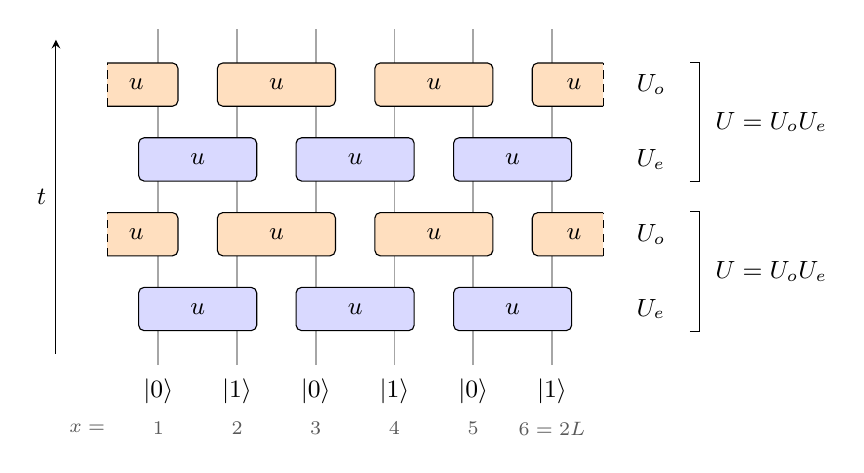
\begin{tikzpicture}[x=1cm,y=0.95cm,
    gate/.style={draw,rounded corners=2pt,minimum height=0.55cm,inner sep=0pt,font=\small},
    ge/.style={gate,fill=blue!15},
    go/.style={gate,fill=orange!25}]
  % wires (time runs upwards)
  \foreach \x in {1,...,6} \draw[gray!70,line width=0.6pt] (\x,0.25) -- (\x,4.75);
  % site labels and initial state
  \foreach \x/\s/\lab in {1/0/1,2/1/2,3/0/3,4/1/4,5/0/5,6/1/{6=2L}}{
    \node[font=\small] at (\x,-0.1) {$|\s\rangle$};
    \node[font=\scriptsize,gray!70!black] at (\x,-0.6) {$\lab$};}
  \node[font=\scriptsize,gray!70!black,anchor=east] at (0.45,-0.6) {$x=$};
  % two time steps
  \foreach \y in {1,3}{
    % even layer: bonds (1,2),(3,4),(5,6)
    \foreach \x in {1,3,5} \node[ge,minimum width=1.5cm] at (\x+0.5,\y) {$u$};
    % odd layer: bonds (2,3),(4,5) and the wrap-around bond (2L,1)
    \foreach \x in {2,4} \node[go,minimum width=1.5cm] at (\x+0.5,\y+1) {$u$};
    \begin{scope}
      \clip (0.35,\y+0.5) rectangle (6.65,\y+1.5);
      \node[go,minimum width=1.5cm] at (0.5,\y+1) {};
      \node[go,minimum width=1.5cm] at (6.5,\y+1) {};
    \end{scope}
    \draw[densely dashed] (0.35,\y+0.71) -- (0.35,\y+1.29) (6.65,\y+0.71) -- (6.65,\y+1.29);
    \node[font=\small] at (0.72,\y+1) {$u$};
    \node[font=\small] at (6.28,\y+1) {$u$};
    % layer labels
    \node[anchor=west,font=\small] at (6.95,\y)   {$\mathbb U_e$};
    \node[anchor=west,font=\small] at (6.95,\y+1) {$\mathbb U_o$};
    \draw (7.75,\y-0.3) -- ++(0.12,0) -- (7.87,\y+1.3) -- ++(-0.12,0);
    \node[anchor=west,font=\small] at (7.95,\y+0.5) {$\mathbb U=\mathbb U_o\mathbb U_e$};
  }
  % time arrow
  \draw[->,>=stealth] (-0.3,0.4) -- (-0.3,4.6) node[midway,left,font=\small] {$t$};
\end{tikzpicture}
\caption{Two time steps of the brickwork circuit, drawn for $L=3$; time runs
upwards. Blue gates form the even layer $\mathbb U_e$ (bonds $(2x+1,2x+2)$), orange
gates the odd layer $\mathbb U_o$ (bonds $(2x,2x+1)$). The two dashed half-gates are
one and the same gate, on the bond $(2L,1)$ that closes the ring.}
\label{fig:Q018-circuit}
\end{figure}
 
\begin{enumerate}[label=\textbf{(\alph*)},leftmargin=*]
  \item \emph{Warm-up, $L=1$.} Here the two bonds coincide, so
        $\mathbb U=u^{2}$. Writing
        $\ket{\pm}:=\tfrac{1}{\sqrt2}\bigl(\ket{01}\pm\ket{10}\bigr)$, show that
        \[
          \ket{\Psi_t}=\frac{e^{i\omega t}\ket{+}+e^{-i\omega t}\ket{-}}{\sqrt2},
        \]
        and deduce that for any observable $\mathcal O$
        \[
          \avg{\Psi_t}{\mathcal O}{\Psi_t}
          =\tfrac12\Bigl\{\avg{+}{\mathcal O}{+}+\avg{-}{\mathcal O}{-}
            +e^{2i\omega t}\avg{-}{\mathcal O}{+}
            +e^{-2i\omega t}\avg{+}{\mathcal O}{-}\Bigr\}.
        \]
 
  \item \emph{Fermionisation, $L>1$.} Define, by the Jordan--Wigner transformation,
        for $x=1,\dots,2L$,
        \[
          c_x=\frac{X_x-iY_x}{2}\prod_{y=1}^{x-1}(-Z_y) ,
          \qquad
          c^{\dagger}_x=\frac{X_x+iY_x}{2}\prod_{y=1}^{x-1}(-Z_y) .
        \]
        These are canonical fermions, $\{c_x,c^{\dagger}_y\}=\delta_{xy}$ and
        $\{c_x,c_y\}=0$, with $c^{\dagger}_xc_x=\tfrac12(\id+Z_x)$: the state $\ket0$
        is the occupied one, and $-Z_y=e^{i\pi c^{\dagger}_yc_y}$. Let
        $\hat N=\sum_{x=1}^{2L}c^{\dagger}_xc_x$ and extend the labelling past the
        last site by the boundary condition
        \[
          c_{2L+1}:=e^{i\pi\hat N}\,c_1 .
        \]
        Show that the two layers become exponentials of quadratic forms,
        \[
          \mathbb U_e=\exp\Bigl[\tfrac{i\omega}{2}\sum_{x=0}^{L-1}
            \bigl(c^{\dagger}_{2x+1}c_{2x+2}+c^{\dagger}_{2x+2}c_{2x+1}\bigr)\Bigr],
          \qquad
          \mathbb U_o=\exp\Bigl[\tfrac{i\omega}{2}\sum_{x=1}^{L}
            \bigl(c^{\dagger}_{2x}c_{2x+1}+c^{\dagger}_{2x+1}c_{2x}\bigr)\Bigr].
        \]
        State explicitly where the Jordan--Wigner strings cancel, and why the boundary
        term depends on the parity of $\hat N$.
 
  \item \emph{Momentum space.} In a sector of fixed $\hat N=N$, define
        \[
          \bar c_k=\frac{1}{\sqrt{2L}}\sum_{n=1}^{2L}e^{ikn}c_n ,
        \]
        \[
          \mathcal S_+\equiv\Bigl\{\tfrac{\pi}{L}\,j+\tfrac{\pi}{2L}\,\mathrm{mod}(N+1,2)
            \;:\; j=0,\dots,L-1\Bigr\},
        \]
        so that $k$ runs over $\mathcal S_+\cup(\mathcal S_+-\pi)$, a set of $2L$
        momenta. Show that each layer becomes block diagonal, mixing only $k$ with
        $k-\pi$:
        \[
          \mathbb U_e=\exp\Bigl[\,\sum_{k\in\mathcal S_+}
            \begin{pmatrix}\bar c^{\dagger}_k&\bar c^{\dagger}_{k-\pi}\end{pmatrix}
            B_k
            \begin{pmatrix}\bar c_k\\ \bar c_{k-\pi}\end{pmatrix}\Bigr],
          \qquad
          \mathbb U_o=\bigl(\text{same with }A_k\bigr),
        \]
        with
        \[
          B_k=A_k^{T}=\tfrac{i\omega}{2}\bigl(\cos(k)\,Z+\sin(k)\,Y\bigr).
        \]
        Here and below $Y,Z$ inside a $2\times2$ block are Pauli matrices acting on
        the mode index $(k,k-\pi)$, not on a qubit. Explain why this particular set
        of momenta is forced, and why $k$ and $k-\pi$ are coupled, and not any other
        pair.
 
  \item \emph{Floquet diagonalisation.} Since both exponents are quadratic, so is their
        Baker--Campbell--Hausdorff combination:
        \[
          \mathbb U=\mathbb U_o\mathbb U_e
          =\exp\Bigl[\,\sum_{k\in\mathcal S_+}
            \begin{pmatrix}\bar c^{\dagger}_k&\bar c^{\dagger}_{k-\pi}\end{pmatrix}
            \log\bigl[e^{A_k}e^{B_k}\bigr]
            \begin{pmatrix}\bar c_k\\ \bar c_{k-\pi}\end{pmatrix}\Bigr].
        \]
        Take as given the $SU(2)$ identity
        \[
          e^{A_k}e^{B_k}
          =e^{-\frac{i}{2}\varphi_kY}\,e^{i\varepsilon_kZ}\,e^{\frac{i}{2}\varphi_kY},
        \]
        with
        \[
          \varphi_k\equiv\arctan\bigl(\tan(\omega/2)\sin k\bigr)
            +\pi\,\theta_{\text{H}}\!\bigl(k-\tfrac{\pi}{2}\bigr),
        \]
        \[
          \tan\varepsilon_k=
            \frac{\sqrt{\sin^{4}(\omega/2)\sin^{2}(2k)+\sin^{2}(\omega)\cos^{2}(k)}}
                 {\cos^{2}(\omega/2)-\sin^{2}(\omega/2)\cos(2k)},
          \qquad \varepsilon_k\in[0,\pi],
        \]
        $\theta_{\text H}$ being the Heaviside step function. (The branch
        $\varepsilon_k\in[0,\pi]$ matters only when the denominator is negative, which
        can happen for $\omega>\pi/2$; there $\varepsilon_k>\pi/2$.) Show that the
        Bogoliubov modes
        \[
          \begin{pmatrix}b_k\\ b_{k-\pi}\end{pmatrix}
          :=e^{\frac{i}{2}\varphi_kY}\begin{pmatrix}\bar c_k\\ \bar c_{k-\pi}\end{pmatrix}
        \]
        diagonalise the propagator,
        \[
          \mathbb U=\exp\Bigl[\,i\sum_{k\in\mathcal S_+}
            \varepsilon_k\bigl(b^{\dagger}_kb_k-b^{\dagger}_{k-\pi}b_{k-\pi}\bigr)\Bigr],
        \]
        and check that $b_k,b^{\dagger}_k$ are again canonical.
 
  \item \emph{Observables.} $\ket{\Psi_0}$ is Gaussian in the $c_x$ and the evolution is
        quadratic, so Wick's theorem holds at all times and every observable is fixed by
        \[
          C_{x,y}=\avg{\Psi_t}{c^{\dagger}_xc_y}{\Psi_t},
          \qquad
          F_{x,y}=\avg{\Psi_t}{c^{\dagger}_xc^{\dagger}_y}{\Psi_t}.
        \]
        Show that
        \begin{align*}
          \avg{\Psi_t}{Z_x}{\Psi_t}
          &=\frac{(-1)^{x}}{L}\sum_{k\in\mathcal S_+}\cos\varphi_k
             \Bigl(e^{-2i\varepsilon_kt}\avg{\Psi_0}{b^{\dagger}_kb_{k-\pi}}{\Psi_0}
             +e^{2i\varepsilon_kt}\avg{\Psi_0}{b^{\dagger}_{k-\pi}b_k}{\Psi_0}\Bigr)\\
          &\quad+\frac{(-1)^{x}}{L}\sum_{k\in\mathcal S_+}\sin\varphi_k
             \Bigl(\avg{\Psi_0}{b^{\dagger}_kb_k}{\Psi_0}
             -\avg{\Psi_0}{b^{\dagger}_{k-\pi}b_{k-\pi}}{\Psi_0}\Bigr)\\
          &=\frac{(-1)^{x+1}}{L}\sum_{k\in\mathcal S_+}
             \Bigl(\cos^{2}\varphi_k\cos(2\varepsilon_kt)+\sin^{2}\varphi_k\Bigr) .
        \end{align*}
        \emph{(Addendum, not in the source.)} Show that $F_{x,y}\equiv 0$ for this
        circuit and this initial state, and identify the symmetry responsible. Comment
        on how the structure of the answer compares with part~(a).
\end{enumerate}
\end{problem}
 
% ============================================================== solutions ===
 
\begin{solution}[Part (a)]
We have that $XX\ket{01}=\ket{10},\quad XX\ket{10}=\ket{01}$, meanwhile,
$YY\ket{01}=i(-i)\ket{10}=\ket{10},\quad YY\ket{10}=(-i)i\ket{01}=\ket{01}$. So the
states $\ket{\pm}$ are eigenstates of the exponent,
\[
  (XX+YY)\ket{\pm}=\pm2\ket{\pm},
\]
thus
\begin{equation}
    u^2\ket{\pm}=\exp\Bigl[\tfrac{i\omega}{2}\bigl(XX+YY\bigr)\Bigr]\ket{\pm}= e^{\pm i\omega}\ket{\pm} .
\end{equation}
\todo{decompose $\ket{\Psi_0}$ in the basis $\ket{\pm}$; expectation value}
and the result follows directly from 
$\ket{01}= \frac{1}{\sqrt{2}}\left( \ket{+} + \ket{-} \right)$
\end{solution}
 
\begin{solution}[Part (b)]
\todo{write up}
\end{solution}
 
\begin{solution}[Part (c)]
\todo{write up}
\end{solution}
 
\begin{solution}[Part (d)]
\todo{write up}
\end{solution}
 
\begin{solution}[Part (e)]
\todo{write up}
\end{solution}
 
\begin{takeaway}
\todo{one or two sentences}
\end{takeaway}
 
\attempt{
  date        = ,
  time        = ,
  difficulty  = ,
  how it went = ,
}
 
\end{entry}
